\chapter{Event Reconstruction}
\label{reconstruction_chapter}

\section{Electron Reconstruction}

Reconstruction of electrons in CMS is complicated by the fact that electrons,
because of their low mass and the high magnetic field causing them to bend,
emit bremsstrahlung photon which must be accounted for. Additionally, the
amount of material in front of ECAL causes many electrons begin showering
before entering ECAL, adding additional scattered energy deposits that must be
included in the final sum. Information about the material in front of ECAL is
given in \FIG~\ref{fig:tracker_material}\cite{cms_tracker_2014}.

\begin{figure}[tb]
    \centering
    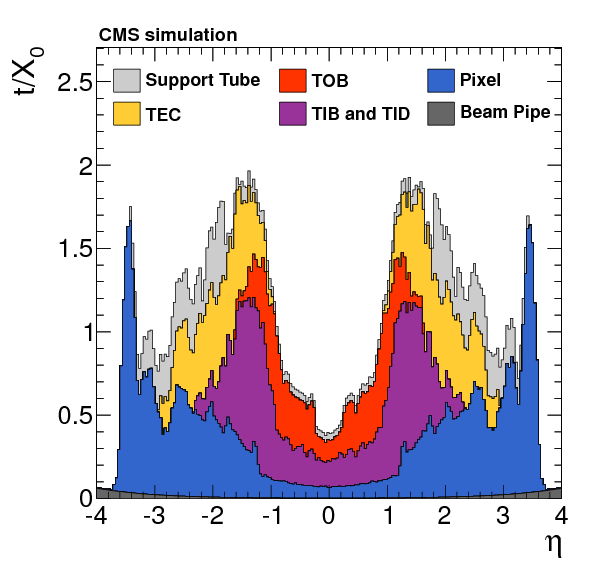
\includegraphics[width=\textwidth]{figures/tracker_material_budget.png}
    \caption{
        The thickness of material, $t$, divided by the radiation length,
        \radiationlength, encountered by particles leaving the nominal
        interaction point before reaching ECAL.
    }
    \label{fig:tracker_material}
\end{figure}

The reconstruction of electrons with $\pt > 20 \GeV$ in CMS starts with an
electron-like cluster of energy in ECAL \cite{eg_reco_2010}. In order to
account for energy lost to bremsstrahlung photons, additional clusters at
constant $\eta$ but changing $\phi$ are added together to form superclusters
\cite{baffioni_2007}.

From these superclusters, a point on the tracker where the electron is likely
to have come from is determined by propagating the energy weighted mean
position of the supercluster back through the magnetic field. This spot is then
used to seed  track finding algorithm in the pixel layer. Hits in the tracker
are searched from starting at the innermost layer and working outward. In order
to account for the changing track shape of the track as the electron loses
energy from interacting with the tracker material, a ``Gaussian Sum Filter''
(GSF) is used \cite{adam_2005}. Low energy electrons ($\ET < 15 \GeV$) are
constructed with \pt from the tracker and \ET from ECAL, but for electrons with
higher energy the ECAL energy alone is used to avoid issues introduced by
possible poor fits in the tracker. The $\eta$ and $\phi$ of all electron
candidates, regardless of energy, is taken from the track.
